\usetikzlibrary{calc}
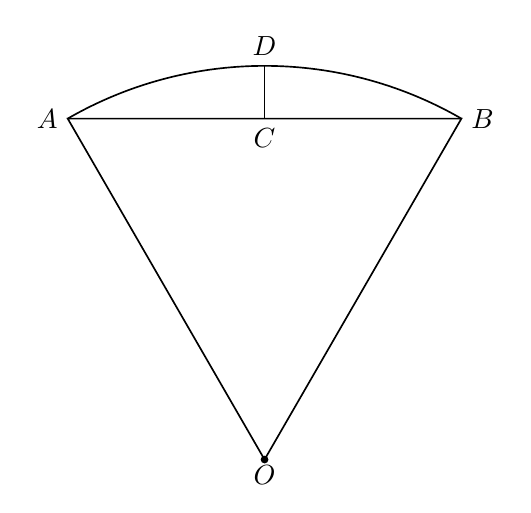
\begin{tikzpicture}[x=2.5cm,y=2.5cm,line width=.6pt,font=\normalsize]
\coordinate (O) at (0,0);
\coordinate (A) at (-1,1.7320508076);
\coordinate (B) at (1,1.7320508076);
\coordinate (C) at (0,1.7320508076);
\coordinate (D) at (0,2);
\draw (O)--(A)--(B)--cycle;
\draw (C)--(D);
\draw (B) arc[start angle=60,end angle=120,radius=5cm];
\node[left] at (A) {$A$};
\node[right] at (B) {$B$};
\node[below] at (C) {$C$};
\node[above] at (D) {$D$};
\node[below=2pt,inner sep=0pt] at (O) {$O$};
\fill (O) circle[radius=1.4pt];
\end{tikzpicture}
